\chapter{Umsetzung}
\section{Design}
\section{Module}
\subsection{Conrad}
Conrad
(\htmladdnormallink{http://www.broadinstitute.org/annotation/conrad/}{http://www.broadinstitute.org/annotation/conrad/})
ist ein \textit{de novo} gene caller, der Genstrukturen wie Exons und Introns
vorhersagen kann.
\index{Conrad} \index{de novo}\index{gene caller}
Die Vorhersage stützt sich dabei auf \textit{semi-Markow Conditional Random
Fields}, kurz \textbf{CRF}.  % wird in hintergründen erwähnt
\index{Markow} \index{Conditional Random Fields} \index{CRF|see{Conditional
Random Fields}}
Conrad benötigt für seine Genvorhersage eine FASTA-Datei mit einer oder
mehreren zu analysierenden DNA-Sequenzen, sowie eine Binärdatei, die Parameter
für den CRF-Alorithmus entält.
Diese Binärdatei wird in einem Trainingslauf erstellt, der vor der
eigentlichen Genvorhersage durchgeführt wird. Hierbei wird der CRF-Algorithmus
auf die Eingabesequenz trainiert, um die Qualität der Genvorhersage
zu maximieren. Dieser Trainingslauf benötigt eine FASTA-Datei mit
DNA-Sequenzen, die Gene enthalten, sowie eine GFF-Datei mit Annotationen zu
diesen Genen.

Um einen Eindruck von der Qualität der Genvorhersage zu gewinnen, wurden
mehrere Trainings- und Vorhersage-Schritte mit einem Beispieldatensatz aus dem
Conrad-Packet durchgeführt, deren Ergebnisse dann kreuzvalidiert wurden.
Der Beispieldatensatz beinhaltete 574 Sequenzen von \texttt{Aspergillus niger},
die dazu im Verhältnis 1:10 in zwei Datensätze A und B aufgeteilt wurden.
Das Training erfolgte mit Datensatz B, die anschliessende Vorhersage wurde für
beide Datensätze durchgeführt.
\index{Aspergillus niger}

Das Ergebnis hieraus war also zum einen eine Vorhersage eben der Gene, mit
denen Conrad zuvor trainiert wurde, zum Anderen eine Vorhersage für unbekannte
Sequenzen, der allerdings ein optimales Training vorrausgegangen war.

\begin{figure}[ht]
	\begin{center}
		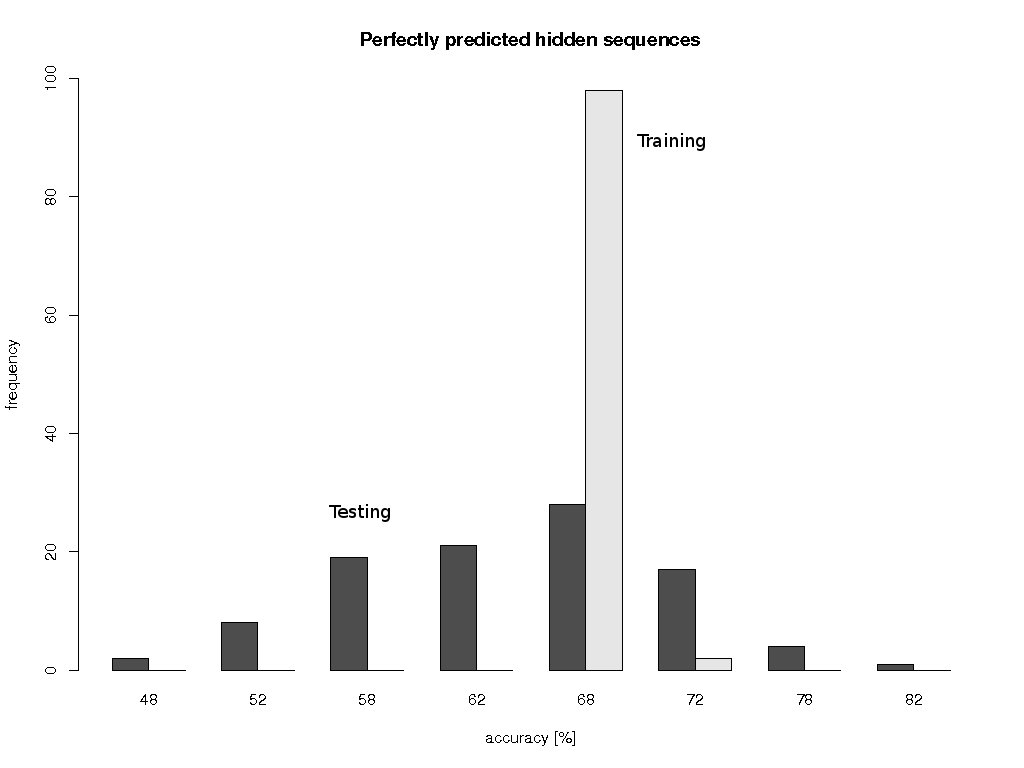
\includegraphics[scale=0.42]{pics/perfectm.jpg}
	\caption{something}
	\end{center}
	\label{fig:perfect}
\end{figure}

\begin{figure}[ht]
	\begin{center}
		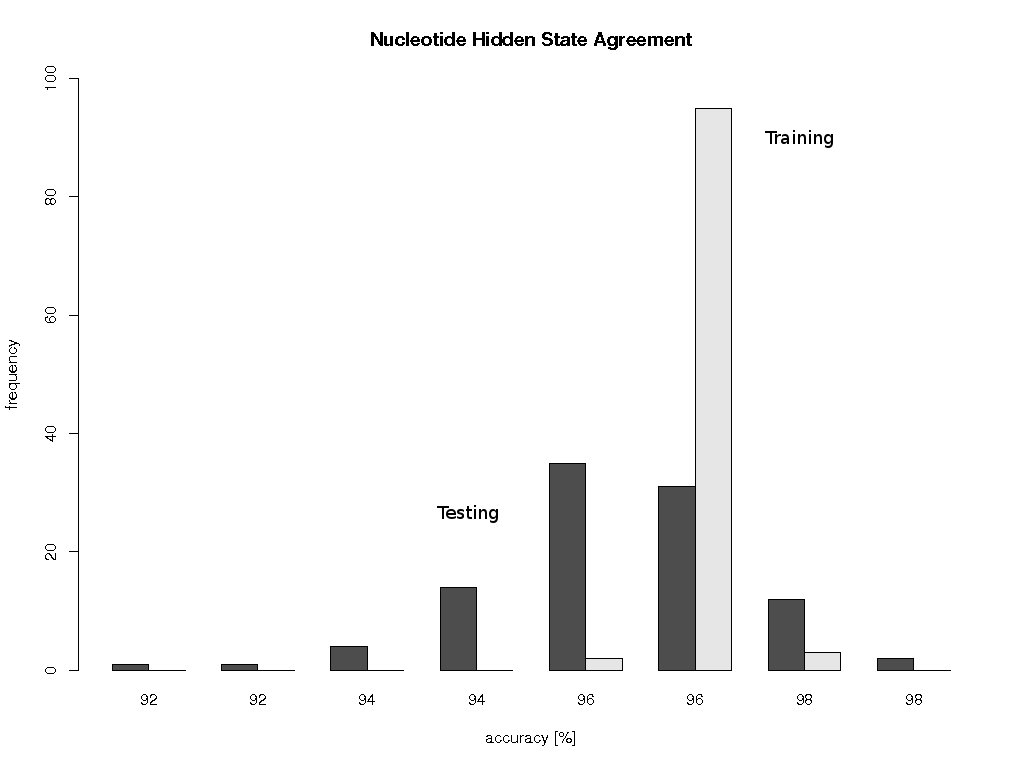
\includegraphics[scale=0.42]{pics/stateAgreementm.jpg}
	\caption{something}
	\end{center}
	\label{fig:stateAgreement}
\end{figure}


